
%{{第二十二回}}{第二十二回}}

\chapter{听曲文宝玉悟禅机\hspace{.5em}制灯谜贾政悲谶语}}

{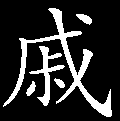
\includegraphics[width=3mm]{../Images/00005}禅理偏成曲调,灯谜巧隐谶言。其中冷暖自寻看,昼夜因循暗转。}

话说贾琏听凤姐儿说有话商量,因止步问是何话。凤姐道:``二十一是薛妹妹的生日,{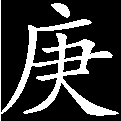
\includegraphics[width=3mm]{../Images/00004}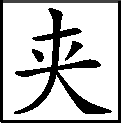
\includegraphics[width=3mm]{../Images/00012}\footnotesize \kaishu 好!}你到底怎么样呢?''贾琏道:``我知道怎么样!你连多少大生日都料理过了,这会子倒没了主意?''凤姐道:``大生日料理,不过是有一定的则例在那里。如今他这生日,大又不是,小又不是,所以和你商量。''{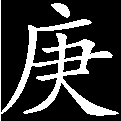
\includegraphics[width=3mm]{../Images/00004}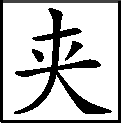
\includegraphics[width=3mm]{../Images/00012}\footnotesize \kaishu 有心机人在此。}贾琏听了,低头想了半日道:``你今儿糊涂了。现有比例,那林妹妹就是例。往年怎么给林妹妹过的,如今也照依给薛妹妹过就是了。''{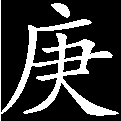
\includegraphics[width=3mm]{../Images/00004}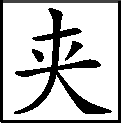
\includegraphics[width=3mm]{../Images/00012}\footnotesize \kaishu 此例引的极是。无怪贾政委以家务也。}凤姐听了,冷笑道:``我难道连这个也不知道?我原也这么想定了。但昨儿听见老太太说,问起大家的年纪生日来,听见薛大妹妹今年十五岁,虽不是整生日,也算得将笄之年。老太太说要替他作生日。想来若果真替他作,自然比往年与林妹妹的不同了。''贾琏道:``既如此,比林妹妹的多增些。''凤姐道:``我也这么想着,所以讨你的口气。我若私自添了东西,你又怪我不告诉明白你了。''贾琏笑道:``罢,罢,这空头情我不领。你不盘察我就够了,我还怪你!''说着,一径去了,不在话下。{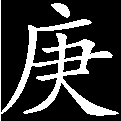
\includegraphics[width=3mm]{../Images/00004}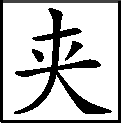
\includegraphics[width=3mm]{../Images/00012}\footnotesize \kaishu 一段题纲写得如见如闻,且不失前篇惧内之旨。最奇者黛玉乃贾母溺爱之人也,不闻为作生辰,却云特意与宝钗,实非人想得着之文也。此书通部皆用此法,瞒过多少见者,余故云不写而写是也。 {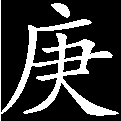
\includegraphics[width=3mm]{../Images/00004}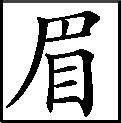
\includegraphics[width=3mm]{../Images/00010}\footnotesize \kaishu 将薛、林作甄玉、贾玉,看书则不失执笔人本旨矣。丁亥夏。畸笏叟。}}

且说史湘云住了两日,因要回去。贾母因说:``等过了你宝姐姐的生日,看了戏再回去。''史湘云听了,只得住下。又一面遣人回去,将自己旧日作的两色针线活计取来,为宝钗生辰之仪。

谁想贾母自见宝钗来了,喜他稳重和平,{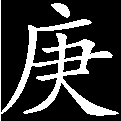
\includegraphics[width=3mm]{../Images/00004}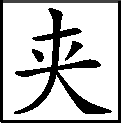
\includegraphics[width=3mm]{../Images/00012}\footnotesize \kaishu 四字评倒黛玉,是以特从贾母眼中写出。}正值他才过第一个生辰,便自己蠲资二十两,{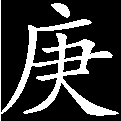
\includegraphics[width=3mm]{../Images/00004}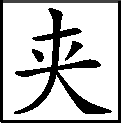
\includegraphics[width=3mm]{../Images/00012}\footnotesize \kaishu 写出太君高兴,世家之常事耳。 {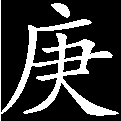
\includegraphics[width=3mm]{../Images/00004}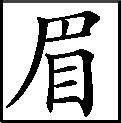
\includegraphics[width=3mm]{../Images/00010}\footnotesize \kaishu 前看凤姐问琏作生日数语甚泛泛,至此见贾母蠲资,方知作者写阿凤心机无丝毫漏笔。己卯冬夜。}}唤了凤姐来,交与他置酒戏。凤姐凑趣笑道:``一个老祖宗给孩子们作生日,{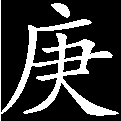
\includegraphics[width=3mm]{../Images/00004}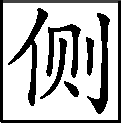
\includegraphics[width=3mm]{../Images/00011}\footnotesize \kaishu 家常话,却是空中楼阁,陡然架起。}不拘怎样,谁还敢争,又办什么酒戏。既高兴要热闹,就说不得自己花上几两。巴巴的找出这霉烂的二十两银子来作东西,这意思还叫我赔上。果然拿不出来也罢了,金的、银的、圆的、扁的,压塌了箱子底,{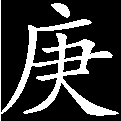
\includegraphics[width=3mm]{../Images/00004}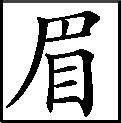
\includegraphics[width=3mm]{../Images/00010}\footnotesize \kaishu 小科诨解颐,却为借当伏线。壬午九月。}只是勒掯我们。举眼看看,谁不是儿女?难道将来只有宝兄弟顶了你老人家上五台山不成?那些梯己只留于他,我们如今虽不配使,也别苦了我们。这个够酒的?够戏的?''说的满屋里都笑起来。贾母亦笑道:``你们听听这嘴!我也算会说的,怎么说不过这猴儿。你婆婆也不敢强嘴,你和我????的。''凤姐笑道:``我婆婆也是一样的疼宝玉,我也没处去诉冤,倒说我强嘴。''说着,又引着贾母笑了一回,{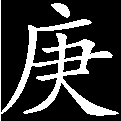
\includegraphics[width=3mm]{../Images/00004}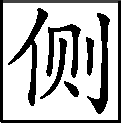
\includegraphics[width=3mm]{../Images/00011}\footnotesize \kaishu 正文在此一句。}贾母十分喜悦。

到晚间,众人都在贾母前,定昏之馀,大家娘儿姊妹等说笑时,贾母因问宝钗爱听何戏,爱吃何物等语。宝钗深知贾母年老人,喜热闹戏文,爱吃甜烂之食,便总依贾母往日素喜者说了出来。{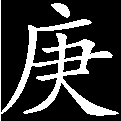
\includegraphics[width=3mm]{../Images/00004}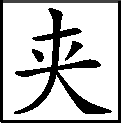
\includegraphics[width=3mm]{../Images/00012}\footnotesize \kaishu 看他写宝钗,比颦儿如何?}贾母更加欢悦。次日便先送过衣服玩物礼去,王夫人、凤姐、黛玉等诸人皆有随分不一,不须多记。

至二十一日,就贾母内院中搭了家常小巧戏台,{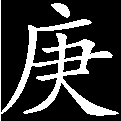
\includegraphics[width=3mm]{../Images/00004}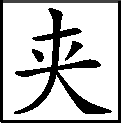
\includegraphics[width=3mm]{../Images/00012}\footnotesize \kaishu 另有大礼所用之戏台也,侯门风俗断不可少。}定了一班新出小戏,昆弋两腔皆有。{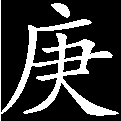
\includegraphics[width=3mm]{../Images/00004}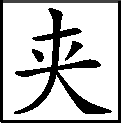
\includegraphics[width=3mm]{../Images/00012}\footnotesize \kaishu 是贾母好热闹之故。}就在贾母上房排了几席家宴酒席,{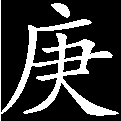
\includegraphics[width=3mm]{../Images/00004}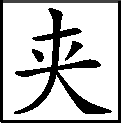
\includegraphics[width=3mm]{../Images/00012}\footnotesize \kaishu 是家宴,非东阁盛设也。非世代公子再想不及此。}并无一个外客,只有薛姨妈、史湘云、宝钗是客,馀者皆是自己人。{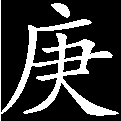
\includegraphics[width=3mm]{../Images/00004}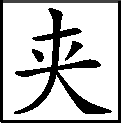
\includegraphics[width=3mm]{../Images/00012}\footnotesize \kaishu 将黛玉亦算为自己人,奇甚!}这日早起,宝玉因不见林黛玉,{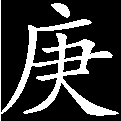
\includegraphics[width=3mm]{../Images/00004}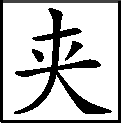
\includegraphics[width=3mm]{../Images/00012}\footnotesize \kaishu 又转至黛玉,文字亦不可少也。}便到他房中来寻,只见林黛玉歪在炕上。宝玉笑道:``起来吃饭去,就开戏了。你爱看那一出?我好点。''林黛玉冷笑道:``你既这样说,你特叫一班戏来,拣我爱的唱给我看。这会子犯不上跐着人借光儿问我。''{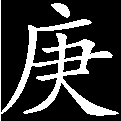
\includegraphics[width=3mm]{../Images/00004}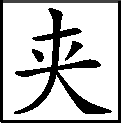
\includegraphics[width=3mm]{../Images/00012}\footnotesize \kaishu 好听之极,令人绝倒。}宝玉笑道:``这有什么难的。明儿就这样行,也叫他们借咱们的光儿。''一面说,一面拉起他来,携手出去吃了饭。

点戏时,贾母一定先叫宝钗点。宝钗推让一遍,无法,只得点了一折《西游记》。{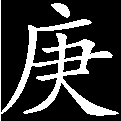
\includegraphics[width=3mm]{../Images/00004}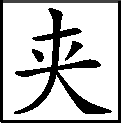
\includegraphics[width=3mm]{../Images/00012}\footnotesize \kaishu 是顺贾母之心也。}贾母自是欢喜,然后便命凤姐点。凤姐亦知贾母喜热闹,更喜谑笑科诨,{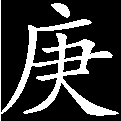
\includegraphics[width=3mm]{../Images/00004}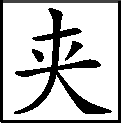
\includegraphics[width=3mm]{../Images/00012}\footnotesize \kaishu 写得周到,想得奇趣,实是必真有之。}便点了一出《刘二当衣》。{{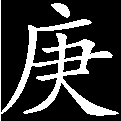
\includegraphics[width=3mm]{../Images/00004}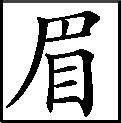
\includegraphics[width=3mm]{../Images/00010}\footnotesize \kaishu 凤姐点戏,脂砚执笔事,今知者{(聊聊)}{[}寥寥{]}矣,不怨夫? 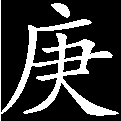
\includegraphics[width=3mm]{../Images/00004}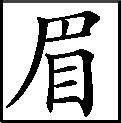
\includegraphics[width=3mm]{../Images/00010}\footnotesize \kaishu 前批``知者寥寥'',今丁亥夏只剩朽物一枚,宁不痛乎!}}贾母果真更又喜欢,然后便命黛玉点。{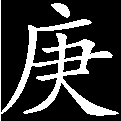
\includegraphics[width=3mm]{../Images/00004}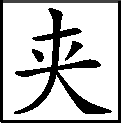
\includegraphics[width=3mm]{../Images/00012}\footnotesize \kaishu 先让凤姐点者,是非待凤先而后玉也。盖亦素喜凤嘲笑得趣之故,今故命彼点,彼亦自知,并不推让,承命一点,便合其意。此篇是贾母取乐,非礼筵大典,故如此写。}黛玉因让薛姨妈王夫人等。贾母道:``今日原是我特带着你们取笑,咱们只管咱们的,别理他们。我巴巴的唱戏摆酒,为他们不成?他们在这里白听白吃,已经便宜了,还让他们点呢!''说着,大家都笑了。黛玉方点了一出。{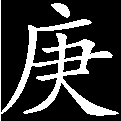
\includegraphics[width=3mm]{../Images/00004}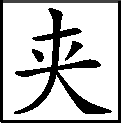
\includegraphics[width=3mm]{../Images/00012}\footnotesize \kaishu 不提何戏,妙!盖黛玉不喜看戏也。正是与后文``妙曲警芳心''留地步,正见此时不过草草随众而已,非心之所愿也。}然后宝玉、史湘云、迎、探、惜、李纨等俱各点了,接出扮演。

至上酒席时,贾母又命宝钗点。宝钗点了一出《鲁智深醉闹五台山》。宝玉道:``只好点这些戏。''宝钗道:``你白听了这几年的戏,那里知道这出戏的好处,排场又好,词藻更妙。''宝玉道:``我从来怕这些热闹。''宝钗笑道:``要说这一出热闹,你还算不知戏呢。{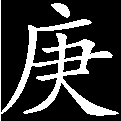
\includegraphics[width=3mm]{../Images/00004}\includegraphics[width=3mm]{../Images/00012}\footnotesize \kaishu 是极!宝钗可谓博学矣,不似黛玉只一《牡丹亭》便心身不自主矣。真有学问如此,宝钗是也。}你过来,我告诉你,这一出戏热闹不热闹。------是一套北《点绛唇》,铿锵顿挫,韵律不用说是好的了,只那词藻中有一支《寄生草》,填的极妙,你何曾知道。''宝玉见说的这般好,便凑近来央告:``好姐姐,念与我听听。''宝钗便念道:

漫揾英雄泪,相离处士家。谢慈悲剃度在莲台下。没缘法转眼分离乍。赤条条来去无牵挂。那里讨烟蓑雨笠卷单行?一任俺芒鞋破钵随缘化!{\includegraphics[width=3mm]{../Images/00004}\includegraphics[width=3mm]{../Images/00012}\footnotesize \kaishu 此阕出自《山门》传奇。近之唱者将``一任俺''改为``早辞却'',无理不通之甚。必从``一任俺''三字,则``随缘''二字方不脱落。}

宝玉听了,喜的拍膝画圈,称赏不已,又赞宝钗无书不知,林黛玉道:``安静看戏罢,还没唱《山门》,你倒《妆疯》了。''{\includegraphics[width=3mm]{../Images/00004}\includegraphics[width=3mm]{../Images/00012}\footnotesize \kaishu 趣极!今古利口莫过于优伶。此一诙谐,优伶亦不得如此急速得趣,可谓才人百技也。一段醋意可知。}说的湘云也笑了。于是大家看戏。

至晚散时,贾母深爱那作小旦的与一个作小丑的,因命人带进来,细看时益发可怜见。{\includegraphics[width=3mm]{../Images/00004}\includegraphics[width=3mm]{../Images/00012}\footnotesize \kaishu 是贾母眼中{(之)}{[}心{]}内之想。}因问年纪,那小旦才十一岁,小丑才九岁,大家叹息一回。贾母令人另拿些肉果与他两个,又另外赏钱两串。凤姐笑道:``这个孩子扮上活像一个人,{\includegraphics[width=3mm]{../Images/00004}\includegraphics[width=3mm]{../Images/00011}\footnotesize \kaishu 明明不叫人说出。}你们再看不出来。''宝钗心里也知道,便只一笑,不肯说。{\includegraphics[width=3mm]{../Images/00004}\includegraphics[width=3mm]{../Images/00012}\footnotesize \kaishu 宝钗如此。}宝玉也猜着了,亦不敢说。{\includegraphics[width=3mm]{../Images/00004}\includegraphics[width=3mm]{../Images/00012}\footnotesize \kaishu ``不敢'',{(少)}{[}妙{]}。}史湘云接着笑道:``倒像林妹妹的模样儿。''{\includegraphics[width=3mm]{../Images/00004}\includegraphics[width=3mm]{../Images/00012}\footnotesize \kaishu 口直心快,无有不可说之事。 {\includegraphics[width=3mm]{../Images/00004}\includegraphics[width=3mm]{../Images/00011}\footnotesize \kaishu 事无不可对人言。 \includegraphics[width=3mm]{../Images/00004}\includegraphics[width=3mm]{../Images/00010}\footnotesize \kaishu 湘云、探春二卿,正``事无不可对人言''之性。丁亥夏。畸笏叟。}}宝玉听了,忙把湘云瞅了一眼,使个眼色。众人却都听了这话,留神细看,都笑起来了,说果然不错。一时散了。

晚间,湘云更衣时,便命翠缕把衣包打开收拾,都包了起来。翠缕道:``忙什么,等去的日子再包不迟。''湘云道:``明儿一早就走。在这里作什么?------看人家的鼻子眼睛,什么意思!''{\includegraphics[width=3mm]{../Images/00004}\includegraphics[width=3mm]{../Images/00012}\footnotesize \kaishu 此是真恼,非颦儿之恼可比,然错怪宝玉矣。亦不可不恼。}宝玉听了这话,忙赶近前拉他说道:``好妹妹,你错怪了我。林妹妹是个多心的人。别人分明知道,不肯说出来,也皆因怕他恼。谁知你不防头就说了出来,他岂不恼你。我是怕你得罪了他,所以才使眼色。你这会子恼我,不但辜负了我,而且反倒委曲了我。若是别人,那怕他得罪了十个人,与我何干呢。''湘云摔手道:``你那花言巧语别哄我。我也原不如你林妹妹,别人说他,拿他取笑都使得,只我说了就有不是。我原不配说他。他是小姐主子,我是奴才丫头,得罪了他,使不得!''宝玉急的说道:``我倒是为你,反为出不是来了。我要有外心,{\includegraphics[width=3mm]{../Images/00004}\includegraphics[width=3mm]{../Images/00011}\footnotesize \kaishu 玉兄急了。}立刻就化成灰,叫万人践踹!''{\includegraphics[width=3mm]{../Images/00004}\includegraphics[width=3mm]{../Images/00012}\footnotesize \kaishu 千古未闻之誓,恳切尽情。宝玉此刻之心为如何?}湘云道:``大正月里,少信嘴胡说。{\includegraphics[width=3mm]{../Images/00004}\includegraphics[width=3mm]{../Images/00011}\footnotesize \kaishu 回护石兄。}这些没要紧的恶誓、散话、歪话,说给那些小性儿、行动爱恼的人,会辖治你的人{\includegraphics[width=3mm]{../Images/00004}\includegraphics[width=3mm]{../Images/00011}\footnotesize \kaishu 此人为谁?}听去!别叫我啐你。''说着,一径至贾母里间,忿忿的躺着去了。

宝玉没趣,只得又来寻黛玉。刚到门槛前,黛玉便推出来,将门关上。宝玉又不解其意,在窗外只是吞声叫``好妹妹''。黛玉总不理他。宝玉闷闷的垂头自审。袭人早知端的,当此时断不能劝。{\includegraphics[width=3mm]{../Images/00004}\includegraphics[width=3mm]{../Images/00012}\footnotesize \kaishu 宝玉在此时一劝必崩了,袭人见机甚妙。}那宝玉只是呆呆的站在那里。

黛玉只当他回房去了,便起来开门,只见宝玉还站在那里。黛玉反不好意思,不好再关,只得抽身上床躺着。宝玉随进来问道:``凡事都有个原故,说出来,人也不委曲。好好的就恼了,终是什么原故起的?''林黛玉冷笑道:``问的我倒好,我也不知为什么原故。我原是给你们取笑的,------拿我比戏子取笑!''宝玉道:``我并没有比你,我并没笑,为什么恼我呢?''黛玉道:``你还要比?你还要笑?你不比不笑,比人比了笑了的还利害呢!''{
\includegraphics[width=3mm]{../Images/00004}\includegraphics[width=3mm]{../Images/00011}\footnotesize \kaishu 可谓``官断十条路''是也。}宝玉听说,无可分辩,不则一声。{\includegraphics[width=3mm]{../Images/00004}\includegraphics[width=3mm]{../Images/00012}\footnotesize \kaishu 何便无言可辩?真令人不解。前文湘云方来,``正言弹妒意''一篇中,颦、玉角口,后收至``褂子''一篇,余已注明不解矣。回思自心、自身是玉、颦之心,则洞然可解,否则无可解也。身非宝玉,则有辩有答;若是宝玉,则再不能辩不能答。何也?总在二人心上想来。 {\includegraphics[width=3mm]{../Images/00004}\includegraphics[width=3mm]{../Images/00010}\footnotesize \kaishu 此书如此等文章多多,不能枚举,机括神思自从天分而有。其毛锥写人口气传神摄魄处,怎不令人拍案称奇叫绝!丁亥夏。畸笏叟。}}

黛玉又道:``这一节还恕得。再你为什么又和云儿使眼色?这安的是什么心?莫不是他和我顽,他就自轻自贱了?他原是公侯的小姐,我原是贫民的丫头,他和我顽,设若我回了口,岂不他自惹人轻贱呢。是这主意不是?这却也是你的好心,只是那一个偏又不领你这好情,一般也恼了。{\includegraphics[width=3mm]{../Images/00004}\includegraphics[width=3mm]{../Images/00012}\footnotesize \kaishu 颦儿自知云儿恼,用心甚矣!}你又拿我作情,倒说我小性儿,{\includegraphics[width=3mm]{../Images/00004}\includegraphics[width=3mm]{../Images/00012}\footnotesize \kaishu 颦儿却又听见,用心甚矣!}行动肯恼。你又怕他得罪了我,我恼他。我恼他,与你何干?他得罪了我,又与你何干?''{\includegraphics[width=3mm]{../Images/00004}\includegraphics[width=3mm]{../Images/00012}\footnotesize \kaishu 问的却极是,但未必心应。若能如此,将来泪尽夭亡已化乌有,世间亦无此一部《红楼梦》矣。 {\includegraphics[width=3mm]{../Images/00004}\includegraphics[width=3mm]{../Images/00010}\footnotesize \kaishu 神工乎,鬼工乎?文思至此尽矣。丁亥夏。畸笏。}}

宝玉见说,方才与湘云私谈,他也听见了。细想自己原为他二人,怕生隙恼,方在中调和,不想并未调和成功,反已落了两处的贬谤。正合着前日所看《南华经》上,有``巧者劳而智者忧,无能者无所求,饱食而遨游,泛若不系之舟'',又曰``山木自寇,{\includegraphics[width=3mm]{../Images/00004}\includegraphics[width=3mm]{../Images/00012}\footnotesize \kaishu 按原注:``山木,漆树也。精脉自出,岂人所使之?故云`自寇',言自相戕贼也。''}源泉自盗''等语。{{\includegraphics[width=3mm]{../Images/00004}\includegraphics[width=3mm]{../Images/00012}\footnotesize \kaishu 源泉味甘,然后人争取之,自寻干涸也,亦如山木意,皆寓人智能聪明多知之害也。前文无心云看《南华经》,不过袭人等恼时,无聊之甚,偶以释闷耳。殊不知用于今日,大解悟大觉迷之功甚矣。市徒见此必云:前日看的是外篇《}胠{箧》,如何今日又知若许篇?然则彼时只曾看外篇数语乎?想其理,自然默默看过几篇,适至外篇,故偶触其机,方续之也。若云只看了那几句便续,则宝玉彼时之心是有意续《庄子》,并非释闷时偶续之也。且更有见前所续,则曰续的不通,更可笑矣。试思宝玉虽愚,岂有安心立意与庄叟争衡哉?且宝玉有生以来,此身此心为诸女儿应酬不暇,眼前多少现成有益之事尚无暇去做,岂忽然要分心于腐言糟粕之中哉?可知除闺阁之外,并无一事是宝玉立意作出来的。大则天地阴阳,小则功名荣枯,以及吟篇琢句,皆是随分触情。偶得之,不喜;失之,不悲。若当作有心,谬矣。只看大观园题咏之文,已算平生得意之句得意之事矣,然亦总不见再吟一句,再题一事,据此可见矣。然后可知前夜是无心顺手拈了一本《庄子》在手,且酒兴{(醮醮)}{[}醺醺{]},芳愁默默,顺手不计工拙,草草一续也。若使顺手拈一本近时鼓词,或如``钟无艳赴会''、``齐太子走国''等草野风邪之传,必亦续之矣。观者试看此批,然后谓余不谬。所以可恨者,彼夜却不曾拈了《山门》一出传奇。若使《山门》在案,彼时拈着,又不知于《寄生草》后续出何等超凡入圣大觉大悟诸语录来。◇黛玉一生是聪明所误,宝玉是多事所误。多事者,情之事也,非世事也。多情曰多事,亦宗《庄》笔而来,盖余亦偏矣,可笑。阿凤是机心所误,宝钗是博识所误,湘云是自爱所误,袭人是好胜所误,皆不能跳出庄叟言外,悲亦甚矣。再笔。}}因此越想越无趣。再细想来,目下不过这两个人,尚未应酬妥协,将来犹欲为何?{\includegraphics[width=3mm]{../Images/00004}\includegraphics[width=3mm]{../Images/00012}\footnotesize \kaishu 看他只这一笔,写得宝玉又如何用心于世道。言闺中红粉尚不能周全,何碌碌僭欲治世待人接物哉?视闺中自然如儿戏,视世道如虎狼矣,谁云不然?}想到其间也无庸分辩回答,自己转身回房来。{\includegraphics[width=3mm]{../Images/00004}\includegraphics[width=3mm]{../Images/00012}\footnotesize \kaishu 颦儿云``与你何干'',宝玉如此一回则曰``与我何干''可也。口虽未出,心已悟矣,但恐不常耳。若常存此念,无此一部书矣。看他下文如何转折。}林黛玉见他去了,便知回思无趣,赌气去了,一言也不曾发,不禁自己越发添了气,{\includegraphics[width=3mm]{../Images/00004}\includegraphics[width=3mm]{../Images/00012}\footnotesize \kaishu 只此一句又勾起波浪。去则去,来则来,又何气哉?总是断不了这根孽肠,忘不了这个祸害,既无而又有也。}便说道:``这一去,一辈子也别来,也别说话。''

宝玉不理,{\includegraphics[width=3mm]{../Images/00004}\includegraphics[width=3mm]{../Images/00012}\footnotesize \kaishu 此是极心死处,将来如何?}回房躺在床上,只是瞪瞪的。袭人深知原委,不敢就说,{\includegraphics[width=3mm]{../Images/00004}\includegraphics[width=3mm]{../Images/00012}\footnotesize \kaishu 一说必崩。 \includegraphics[width=3mm]{../Images/00005}\includegraphics[width=3mm]{../Images/00012}\footnotesize \kaishu 一说就恼。}只得以他事来解释,因说道:``今儿看了戏,又勾出几天戏来。宝姑娘一定要还席的。''宝玉冷笑道:``他还不还,管谁什么相干。''{\includegraphics[width=3mm]{../Images/00004}\includegraphics[width=3mm]{../Images/00012}\footnotesize \kaishu 大奇大神之文。此``相干''之语仍是近文与颦儿之语之``相干''也。上文来说,终存于心,却于宝钗身上发泄。素厚者唯颦、云,今为彼等尚存此心,况于素不契者有不直言者乎?情理笔墨,无不尽矣。}袭人见这话不是往日的口吻,因又笑道:``这是怎么说?好好的大正月里,娘儿们姊妹们都喜喜欢欢的,你又怎么这个形景了?''宝玉冷笑道:``他们娘儿们姊妹们欢喜不欢喜,也与我无干。''{\includegraphics[width=3mm]{../Images/00004}\includegraphics[width=3mm]{../Images/00012}\footnotesize \kaishu 先及宝钗,后及众人,皆一颦之祸流毒于众人。宝玉之心实仅有一颦乎?}袭人笑道:``他们既随和,你也随和,岂不大家彼此有趣。''宝玉道:``什么是`大家彼此'!他们有`大家彼此',我是`赤条条来去无牵挂'。''{\includegraphics[width=3mm]{../Images/00004}\includegraphics[width=3mm]{../Images/00012}\footnotesize \kaishu 拍案叫好!当此一发,西方诸佛亦来听此棒喝,参此语录。}谈及此句,不觉泪下。{\includegraphics[width=3mm]{../Images/00004}\includegraphics[width=3mm]{../Images/00012}\footnotesize \kaishu 还是心中不净、不了,斩不断之故。}袭人见此光景,不肯再说。宝玉细想这句趣味,不禁大哭起来,{\includegraphics[width=3mm]{../Images/00004}\includegraphics[width=3mm]{../Images/00012}\footnotesize \kaishu 此是忘机大悟,世人所谓疯癫是也。}翻身起来至案,遂提笔立占一偈云:

你证我证,心证意证。

是无有证,斯可云证。

无可云证,是立足境。{\includegraphics[width=3mm]{../Images/00004}\includegraphics[width=3mm]{../Images/00012}\footnotesize \kaishu 已悟已觉,是好偈矣。◇宝玉悟禅亦由情,读书亦由情,读《庄》亦由情。可笑。}

写毕,自虽解悟,又恐人看此不解,{\includegraphics[width=3mm]{../Images/00004}\includegraphics[width=3mm]{../Images/00012}\footnotesize \kaishu 自悟则自了,又何用人亦解哉?此正是犹未正觉大悟也。}因此亦填一支《寄生草》,也写在偈后。{\includegraphics[width=3mm]{../Images/00004}\includegraphics[width=3mm]{../Images/00012}\footnotesize \kaishu 此处亦续《寄生草》。余前批云不曾见续,今却见之,是意外之幸也。盖前夜《庄子》是道悟,此日是禅悟,天花散漫之文也。}自己又念一遍,自觉无挂碍,中心自得,便上床睡了。{\includegraphics[width=3mm]{../Images/00004}\includegraphics[width=3mm]{../Images/00012}\footnotesize \kaishu 前夜已悟,今夜又悟,二次翻身不出,故一世堕落无成也。不写出曲文何辞,却留于宝钗眼中写出,是交代过节也。}

谁想黛玉见宝玉此番果断而去,故以寻袭人为由,来视动静。{\includegraphics[width=3mm]{../Images/00004}\includegraphics[width=3mm]{../Images/00012}\footnotesize \kaishu 这又何必?总因慧刀不利,未斩毒龙之故也。大都如此,叹叹!}袭人笑回:``已经睡了。''黛玉听说,便要回去。袭人笑道:``姑娘请站住,有一个字帖儿,瞧瞧是什么话。''说着,便将方才那曲子与偈语悄悄拿来,递与黛玉看。黛玉看了,知是宝玉一时感忿而作,不觉可笑可叹,{\includegraphics[width=3mm]{../Images/00004}\includegraphics[width=3mm]{../Images/00012}\footnotesize \kaishu 是个善知觉。何不趁此大家一解,齐证上乘,甘心堕落迷津哉?}便向袭人道:``作的是玩意儿,无甚关系。''{\includegraphics[width=3mm]{../Images/00004}\includegraphics[width=3mm]{../Images/00012}\footnotesize \kaishu 黛玉说``无关系'',将来必无关系。◇余正恐颦、玉从此一悟,则无妙文可看矣。不想颦儿视之为漠然,更曰``无关系'',可知宝玉不能悟也。余心稍慰。盖宝玉一生行为,颦知最确,故余闻语则信而又信,不必定玉而后证之方信也。◇余云恐他二人一悟则无妙文可看,然欲为开我怀,为醒我目,却愿他二人永堕迷津,生出孽障,余心甚不公矣。世云损人利己者,余此愿是矣。试思之,可发一笑。今自呈于此,亦可为后人一笑,以助茶前酒后之兴耳。而今后天地间岂不又添一趣谈乎?凡书皆以趣谈读去,其理自明,其趣自得矣。}说毕,便携了回房去,与湘云同看。{\includegraphics[width=3mm]{../Images/00004}\includegraphics[width=3mm]{../Images/00012}\footnotesize \kaishu 却不同湘云分崩,有趣!}次日又与宝钗看。宝钗看其词{\includegraphics[width=3mm]{../Images/00004}\includegraphics[width=3mm]{../Images/00012}\footnotesize \kaishu 出自宝钗目中,正是大关键处。}曰:

无我原非你,从他不解伊。肆行无碍凭来去。茫茫着甚悲愁喜,纷纷说甚亲疏密。从前碌碌却因何,{到如今}回头试想真无趣!{\includegraphics[width=3mm]{../Images/00004}\includegraphics[width=3mm]{../Images/00012}\footnotesize \kaishu 看此一曲,试思作者当日发愿不作此书,却立意要作传奇,则又不知有如何词曲矣。}

看毕,又看那偈语,又笑道:``这个人悟了。都是我的不是,都是我昨儿一支曲子惹出来的。这些道书禅机最能移性。{\includegraphics[width=3mm]{../Images/00004}\includegraphics[width=3mm]{../Images/00012}\footnotesize \kaishu 拍案叫绝!此方是大悟彻语录,非宝卿不能谈此也。}明儿认真说起这些疯话来,存了这个意思,都是从我这一只曲子上来,我成了个罪魁了。''说着,便撕了个粉碎,递与丫头们说:``快烧了罢。''黛玉笑道:``不该撕,等我问他。你们跟我来,包管叫他收了这个痴心邪话。''

三人果然都往宝玉屋里来。一进来,黛玉便笑道:``宝玉,我问你:至贵者是`宝',至坚者是`玉'。尔有何贵?尔有何坚?''{\includegraphics[width=3mm]{../Images/00004}\includegraphics[width=3mm]{../Images/00012}\footnotesize \kaishu 拍案叫绝!大和尚来答此机锋,想亦不能答也。非颦儿,第二人无此灵心慧性也。}宝玉竟不能答。三人拍手笑道:``这样钝愚,还参禅呢。''黛玉又道:``你那偈末云:`无可云证,是立足境。'固然好了,只是据我看,还未尽善。我再续两句在后。''因念云:``无立足境,是方干净。''{\includegraphics[width=3mm]{../Images/00004}\includegraphics[width=3mm]{../Images/00012}\footnotesize \kaishu 拍案叫绝!此又深一层也。亦如谚云:``去年贫,只立锥;今年贫,锥也无。''其理一也。}宝钗道:``实在这方悟彻。当日南宗六祖惠能,{\includegraphics[width=3mm]{../Images/00004}\includegraphics[width=3mm]{../Images/00010}\footnotesize \kaishu 用得妥当之极!}初寻师至韶州,闻五祖弘忍在黄梅,他便充役火头僧。五祖欲求法嗣,令徒弟诸僧各出一偈。上座神秀说道:`身是菩提树,心如明镜台,时时勤拂拭,莫使有尘埃。'彼时惠能在厨房碓米,听了这偈,说道:`美则美矣,了则未了。'因自念一偈曰:`菩提本非树,明镜亦非台,本来无一物,何处惹尘埃?'五祖便将衣钵传他。{\includegraphics[width=3mm]{../Images/00004}\includegraphics[width=3mm]{../Images/00012}\footnotesize \kaishu 出《语录》。总写宝卿博学宏览,胜诸才人;颦儿却聪慧灵智,非学力所致------皆绝世绝伦之人也。宝玉宁不愧杀!}今儿这偈语,亦同此意了。只是方才这句机锋,尚未完全了结,这便丢开手不成?''黛玉笑道:``彼时不能答,就算输了,这会子答上了也不为出奇。只是以后再不许谈禅了。连我们两个所知所能的,你还不知不能呢,还去参禅呢。''宝玉自己以为觉悟,不想忽被黛玉一问,便不能答,宝钗又比出``语录''来,此皆素不见他们能者。自己想了一想:``原来他们比我的知觉在先,尚未解悟,我如今何必自寻苦恼。''{\includegraphics[width=3mm]{../Images/00004}\includegraphics[width=3mm]{../Images/00010}\footnotesize \kaishu 前以《庄子》为引,故偶续之。又借颦儿诗一鄙驳,兼不写着落,以为瞒过看官矣。此回用若许曲折,仍用老庄引出一偈来,再续一《寄生草》,可谓大觉大悟矣。以之上承果位,以后无书可作矣。却又轻轻用黛玉一问机锋,又续偈言二句,并用宝钗讲五祖六祖问答二实偈子,使宝玉无言可答,仍将一大善知识,始终跌不出警幻幻榜中,作下回若干回书。真有机心游龙不测之势,安得不叫绝?且历来小说中万写不到者。己卯冬夜。}想毕,便笑道:``谁又参禅,不过一时顽话罢了。''说着,四人仍复如旧。{\includegraphics[width=3mm]{../Images/00004}\includegraphics[width=3mm]{../Images/00012}\footnotesize \kaishu 轻轻抹去也。``心净难''三字不谬。}

忽然人报,娘娘差人送出一个灯谜儿,命你们大家去猜,猜着了每人也作一个进去。四人听说忙出去,至贾母上房。只见一个小太监,拿了一盏四角平头白纱灯,专为灯谜而制,上面已有一个,众人都争看乱猜。小太监又下谕道:``众小姐猜着了,不要说出来,每人只暗暗的写在纸上,一齐封进宫去,娘娘自验是否。''宝钗等听了,近前一看,是一首七言绝句,并无甚新奇,口中少不得称赞,只说难猜,故意寻思,其实一见就猜着了。宝玉、黛玉、湘云、探春{\includegraphics[width=3mm]{../Images/00004}\includegraphics[width=3mm]{../Images/00012}\footnotesize \kaishu 此处透出探春,正是草蛇灰线,后文方不突然。}四个人也都解了,各自暗暗的写了半日。一并将贾环、贾兰等传来,一齐各揣机心都猜了,{\includegraphics[width=3mm]{../Images/00004}\includegraphics[width=3mm]{../Images/00012}\footnotesize \kaishu 写出猜谜人形景,看他偏于两次{(戒)}{[}禅{]}机后,写此机心机事,足见用意至深至远。}写在纸上。然后各人拈一物作成一谜,恭楷写了,挂在灯上。

太监去了,至晚出来传谕:``前娘娘所制,俱已猜着,惟二小姐与三爷猜的不是。{\includegraphics[width=3mm]{../Images/00004}\includegraphics[width=3mm]{../Images/00012}\footnotesize \kaishu 迎春、贾环也。交错有法。}小姐们作的也都猜了,不知是否。''说着,也将写的拿出来。也有猜着的,也有猜不着的,都胡乱说猜着了。太监又将颁赐之物送与猜着之人,每人一个宫制诗筒,{\includegraphics[width=3mm]{../Images/00004}\includegraphics[width=3mm]{../Images/00012}\footnotesize \kaishu 诗筒,身边所佩之物,以待偶成之句草录暂收之,其归至窗前不致有忘也。或茜牙成,或琢香屑,或以绫素为之,不一,想来奇特事,从不知也。}一柄茶筅,{\includegraphics[width=3mm]{../Images/00004}\includegraphics[width=3mm]{../Images/00012}\footnotesize \kaishu 破竹如帚,以净茶具之积也。◇二物极微极雅。}独迎春、贾环二人未得。迎春自为顽笑小事,并不介意,{\includegraphics[width=3mm]{../Images/00004}\includegraphics[width=3mm]{../Images/00012}\footnotesize \kaishu 大家小姐。}贾环便觉得没趣。且又听太监说:``三爷说的这个不通,娘娘也没猜,叫我带回问三爷是个什么。''众人听了,都来看他作的什么,写道是:

大哥有角只八个,二哥有角只两根。

大哥只在床上坐,二哥爱在房上蹲。{\includegraphics[width=3mm]{../Images/00004}\includegraphics[width=3mm]{../Images/00012}\footnotesize \kaishu 可发一笑,真环哥之谜。◇诸卿勿笑,难为了作者摹拟。}

众人看了,大发一笑。贾环只得告诉太监说:``一个枕头,一个兽头。''{\includegraphics[width=3mm]{../Images/00004}\includegraphics[width=3mm]{../Images/00012}\footnotesize \kaishu 亏他好才情,怎么想来?}太监记了,领茶而去。

贾母见元春这般有兴,自己越发喜乐,便命速作一架小巧精致围屏灯来,设于当屋,命他姊妹各自暗暗的作了,写出来粘于屏上,然后预备下香茶细果以及各色玩物,为猜着之贺。贾政朝罢,见贾母高兴,况在节间,晚上也来承欢取乐。设了酒果,备了玩物,上房悬了彩灯,请贾母赏灯取乐。上面贾母、贾政、宝玉一席,下面王夫人、宝钗、黛玉、湘云又一席,迎、探、惜三个又一席。地下婆娘丫鬟站满。李宫裁、王熙凤二人在里间又一席。{\includegraphics[width=3mm]{../Images/00004}\includegraphics[width=3mm]{../Images/00011}\footnotesize \kaishu 细致。}贾政因不见贾兰,便问:``怎么不见兰哥?''{\includegraphics[width=3mm]{../Images/00004}\includegraphics[width=3mm]{../Images/00012}\footnotesize \kaishu 看他透出贾政极爱贾兰。}地下婆娘忙进里间问李氏,李氏起身笑着回道:``他说方才老爷并没去叫他,他不肯来。''婆娘回复了贾政。众人都笑说:``天生的牛心古怪。''贾政忙遣贾环与两个婆娘将贾兰唤来。贾母命他在身旁坐了,抓果品与他吃。大家说笑取乐。

往常间只有宝玉长谈阔论,今日贾政在这里,便惟有唯唯而已。{\includegraphics[width=3mm]{../Images/00004}\includegraphics[width=3mm]{../Images/00012}\footnotesize \kaishu 写宝玉如此。非世家曾经严父之训者,断写不出此一句。}馀者湘云虽系闺阁弱女,却素喜谈论,今日贾政在席,也自缄口禁言。{\includegraphics[width=3mm]{../Images/00004}\includegraphics[width=3mm]{../Images/00012}\footnotesize \kaishu 非世家经明训者,断不知此一句。写湘云如此。}黛玉本性懒与人共,原不肯多语。{\includegraphics[width=3mm]{../Images/00004}\includegraphics[width=3mm]{../Images/00012}\footnotesize \kaishu 黛玉如此。与人多话则不肯,岂得与宝玉话{(更)}{[}便{]}多哉?}宝钗原不妄言轻动,便此时亦是坦然自若。{\includegraphics[width=3mm]{../Images/00004}\includegraphics[width=3mm]{../Images/00012}\footnotesize \kaishu 瞧他写宝钗,真是又曾经严父慈母之明训,又是世府千金,自己又天性从礼合节,前三人之长并归一身。前三人{(向)}{[}尚{]}有捏作之态,故唯宝钗一人作坦然自若,亦不见逾规越矩也。}故此一席虽是家常取乐,反见拘束不乐。{\includegraphics[width=3mm]{../Images/00004}\includegraphics[width=3mm]{../Images/00012}\footnotesize \kaishu 非世家公子断写不及此。想近时之家,纵其儿女哭笑索饮,长者反以为乐,其无礼不法,何如是耶!}贾母亦知因贾政一人在此所致之故,{\includegraphics[width=3mm]{../Images/00004}\includegraphics[width=3mm]{../Images/00012}\footnotesize \kaishu 这一句又明补出贾母亦是世家明训之千金也,不然断想不及此。}酒过三巡,便撵贾政去歇息。贾政亦知贾母之意,撵了自己去后,好让他们姊妹兄弟取乐的。贾政忙陪笑道:``今日原听见老太太这里大设春灯雅谜,故也备了彩礼酒席,特来入会。何疼孙子孙女之心,便不略赐以儿子半点?''{\includegraphics[width=3mm]{../Images/00004}\includegraphics[width=3mm]{../Images/00012}\footnotesize \kaishu 贾政如此,余亦泪下。}贾母笑道:``你在这里,他们都不敢说笑,没的倒叫我闷。你要猜谜时,我便说一个你猜,猜不着是要罚的。''贾政忙笑道:``自然要罚。若猜着了,也是要领赏的。''贾母道:``这个自然。''说着便念道:

猴子身轻站树梢。{\includegraphics[width=3mm]{../Images/00004}\includegraphics[width=3mm]{../Images/00012}\footnotesize \kaishu 所谓``树倒猢狲散''是也。}打一果名。

贾政已知是荔枝,{\includegraphics[width=3mm]{../Images/00004}\includegraphics[width=3mm]{../Images/00012}\footnotesize \kaishu 的是贾母之谜。}便故意乱猜别的,罚了许多东西,然后方猜着,也得了贾母的东西。然后也念一个与贾母猜,念道:

身自端方,体自坚硬。虽不能言,有言必应。{\includegraphics[width=3mm]{../Images/00004}\includegraphics[width=3mm]{../Images/00012}\footnotesize \kaishu 好极!的是贾老之谜,包藏贾府祖宗自身,``必''字隐``笔''字。妙极,妙极!}打一用物。

说毕,便悄悄的说与宝玉。宝玉意会,又悄悄的告诉了贾母。贾母想了想,{\includegraphics[width=3mm]{../Images/00004}\includegraphics[width=3mm]{../Images/00011}\footnotesize \kaishu 太君身份。}果然不差,便说:``是砚台。''贾政笑道:``到底是老太太,一猜就是。''回头说:``快把贺彩送上来。''地下妇女答应一声,大盘小盘一齐捧上。贾母逐件看去,都是灯节下所用所顽新巧之物,甚喜,遂命:``给你老爷斟酒。''宝玉执壶,迎春送酒。贾母因说:``你瞧瞧那屏上,都是他姊妹们做的,再猜一猜我听。''贾政答应,起身走至屏前,只见头一个写道是:

能使妖魔胆尽摧,身如束帛气如雷。

一声震得人方恐,回首相看已化灰。{\includegraphics[width=3mm]{../Images/00004}\includegraphics[width=3mm]{../Images/00012}\footnotesize \kaishu 此元春之谜。才得侥幸,奈寿不长,深可悲哉!}

贾政道:``这是炮竹嗄。''宝玉答道:``是。''贾政又看道:

天运人功理不穷,有功无运也难逢。

因何镇日纷纷乱,只为阴阳数不同。{\includegraphics[width=3mm]{../Images/00004}\includegraphics[width=3mm]{../Images/00012}\footnotesize \kaishu 此迎春一生遭际,惜不得其夫何!}

贾政道:``是算盘。''迎春笑道:``是。''又往下看是:

阶下儿童仰面时,清明妆点最堪宜。

游丝一断浑无力,莫向东风怨别离。{\includegraphics[width=3mm]{../Images/00004}\includegraphics[width=3mm]{../Images/00012}\footnotesize \kaishu 此探春远适之谶也。使此人不远去,将来事败,诸子孙不致流散也,悲哉伤哉!}

贾政道:``这是风筝。''探春笑道:``是。''又看道是:

前身色相总无成,不听菱歌听佛经。

莫道此生沉黑海,性中自有大光明。{\includegraphics[width=3mm]{../Images/00004}\includegraphics[width=3mm]{../Images/00012}\footnotesize \kaishu 此惜春为尼之谶也。公府千金至缁衣乞食,宁不悲夫! {\includegraphics[width=3mm]{../Images/00004}\includegraphics[width=3mm]{../Images/00010}\footnotesize \kaishu 此后破失,俟再补。}}\href{../Text/part0026_split_000.html\#lnkback_1_a}{\textsuperscript{①}}

{  \includegraphics[width=3mm]{../Images/00004}暂记宝钗制谜云:朝罢谁携两袖烟,琴边衾里总无缘。晓筹不用鸡人报,五夜无烦侍女添。焦首朝朝还暮暮,煎心日日复年年。光阴荏苒须当惜,风雨阴晴任变迁。此回未成而芹逝矣,叹叹!丁亥夏。畸笏叟。}

贾政道:``这是佛前海灯嗄。''惜春笑答道:``是海灯。''

贾政心内沉思道:``娘娘所作爆竹,此乃一响而散之物。迎春所作算盘,是打动乱如麻。探春所作风筝,乃飘飘浮荡之物。惜春所作海灯,一发清净孤独。今乃上元佳节,如何皆作此不祥之物为戏耶?''心内愈思愈闷,因在贾母之前,不敢形于色,只得仍勉强往下看去。只见后面写着七言律诗一首,却是宝钗所作,随念道:

朝罢谁携两袖烟,琴边衾里总无缘。

晓筹不用鸡人报,五夜无烦侍女添。

焦首朝朝还暮暮,煎心日日复年年。

光阴荏苒须当惜,风雨阴晴任变迁。

贾政看完,心内自忖道:``此物还倒有限。只是小小之人作此词句,更觉不祥,皆非永远福寿之辈。''想到此处,愈觉烦闷,大有悲戚之状,因而将适才的精神减去十分之八九,只垂头沉思。

贾母见贾政如此光景,想到或是他身体劳乏亦未可定,又兼之恐拘束了众姊妹不得高兴顽耍,即对贾政云:``你竟不必猜了,去安歇罢。让我们再坐一会,也好散了。''贾政一闻此言,连忙答应几个``是''字,又勉强劝了贾母一回酒,方才退出去了。回至房中只是思索,翻来覆去竟难成寐,不由伤悲感慨,不在话下。

且说贾母见贾政去了,便道:``你们可自在乐一乐罢。''一言未了,早见宝玉跑至围屏灯前,指手画脚,满口批评,这个这一句不好,那一个破的不恰当,如同开了锁的猴子一般。宝钗便道:``还像适才坐着,大家说说笑笑,岂不斯文些儿。''凤姐自里间忙出来插口道:``你这个人,就该老爷每日令你寸步不离方好。适才我忘了,为什么不当着老爷,撺掇叫你也作诗谜儿。若果如此,怕不得这会子正出汗呢。''说的宝玉急了,扯着凤姐儿,扭股儿糖似的只是厮缠。贾母又与李宫裁并众姊妹说笑了一会,也觉有些困倦起来。听了听已是漏下四鼓,命将食物撤去,赏散与众人,随起身道:``我们安歇罢。明日还是节下,该当早起。明日晚间再玩罢。''且听下回分解。

{\includegraphics[width=3mm]{../Images/00005}总评:作者具菩提心,捉笔现身说法,每于言外警人再三再四。而读者但以小说古词目之,则大罪过。其先以庄子为引,及偈曲句作醒悟之语,以警觉世人。犹恐不入,再以灯谜伸词致意,自解自叹,以不成寐为言,其用心之切之诚,读者忍不留心而慢忽之耶?}

{\href{../Text/part0026_split_000.html\#navto_1_a}{①}按:底本本回至此止(列本同),后另页书``暂记宝钗制谜\ldots{}\ldots{}''。以下补文有不同版本,均为后人所补,兹据戚本(蒙、舒本略同)。甲辰本补文将``更香''谜归于黛玉,另补入宝钗``竹夫人''谜和宝玉``镜''谜,情节甚不合理,不再附录。}
